\documentclass[final,hyperref={pdfpagelabels=false}]{beamer}
\usepackage{grffile}
\mode<presentation>{\usetheme{PosterLogProb}}
%\mode<presentation>{\usetheme{I6pd2}}
\usepackage[portuguese,brazil]{babel}
\usepackage[latin1]{inputenc}
\usepackage{amsmath,amsthm, amssymb, latexsym}
\usepackage{epsfig}

%\usepackage{algorithm}
%\usepackage{algorithmic}

%\usepackage{times}\usefonttheme{professionalfonts}  % obsolete
%\usefonttheme[onlymath]{serif}
%\boldmath
\usepackage[orientation=portrait,size=a0,scale=1.4,debug]{beamerposter}
% change list indention level
% \setdefaultleftmargin{3em}{}{}{}{}{}
\providecommand\thispdfpagelabel[1]{}
\setbeamertemplate{bibliography entry title}{\color{black}}
\setbeamertemplate{bibliography entry location}{}
\setbeamertemplate{bibliography entry note}{}


%\usepackage{snapshot} % will write a .dep file with all dependencies, allows for easy bundling

\usepackage{array,booktabs,tabularx}
\newcolumntype{Z}{>{\centering\arraybackslash}X} % centered tabularx columns
\newcommand{\pphantom}{\textcolor{ta3aluminium}} % phantom introduces a vertical space in p formatted table columns??!!

\listfiles

\usepackage{amsthm}
%%%%%%%%%%%%%%%%%%%%%%%%%%%%%%%%%%%%%%%%%%%%%%%%%%%%%%%%%%%%%%%%%%%%%%%%%%%%%%%%%%%%%%


 \title{\huge\bfseries\hspace*{-1em} Free and Open Source Software Development and Research:
Opportunities for Software Engineering}
\date{}
\author{\large Fabio Kon
  \and Paulo Meirelles
  \and Antonio Terceiro \\
  \and Christina Chavez
  \and Nelson Lago
  \and Manoel Mendon�a
}
\institute[USP/UFBA]{University of S�o Paulo and Federal University of Bahia, Brazil}

%%%%%%%%%%%%%%%%%%%%%%%%%%%%%%%%%%%%%%%%%%%%%%%%%%%%%%%%%%%%%%%%%%%%%%%%%%%%%%%%%%%%%%
\newlength{\columnheight}
\setlength{\columnheight}{105cm}


%%%%%%%%%%%%%%%%%%%%%%%%%%%%%%%%%%%%%%%%%%%%%%%%%%%%%%%%%%%%%%%%%%%%%%%%%%%%%%%%%%%%%%
\begin{document}
\begin{frame}
  \begin{columns}
    % ---------------------------------------------------------%
    % Set up a column 
    \begin{column}{.49\textwidth}
      \begin{beamercolorbox}[center,wd=\textwidth]{postercolumn}
        \begin{minipage}[T]{.95\textwidth}  % tweaks the width, makes a new \textwidth
          \parbox[t][\columnheight]{\textwidth}{ % must be some better way to set the the height, width and textwidth simultaneously
            % Since all columns are the same length, it is all nice and tidy.  You have to get the height empirically
            % ---------------------------------------------------------%
            % fill each column with content
%\vfill
\begin{block}{Software Engineering research}
  \begin{itemize}
	\item Advancing our understanding of the process of software development
              and its outcomes
        \item Should be based on the study of existing real-world software
        \item FLOSS offers SE researchers the opportunity of basing their
              research on abundant and publicly available data, freely accessible
              data analysis, and software

        \begin{itemize}
	      \item These are basic building blocks for reproducible and
                    extensible science
        \end{itemize}
  \end{itemize}              
\end{block}

%-------------------------------------------------------------------------------
\vfill
\begin{block}{Why FLOSS?}
	\begin{itemize}
		\item Based on a collaborative, efficient, and open development process

		\item Allows users to use, study, modify, and redistribute the software

		\item Centered around some publicly-accessible source code 

		\item Benefits from social, ethical, technical, and economic
                      points of view
		\item Source code access and sharing eases learning and promotes
                      participation in the development of software
		\item Development model that may result in high quality code that
                      gets adapted quickly to different situations with lower
                      direct costs
	\end{itemize}

	\begin{figure}
	  \begin{center}
	    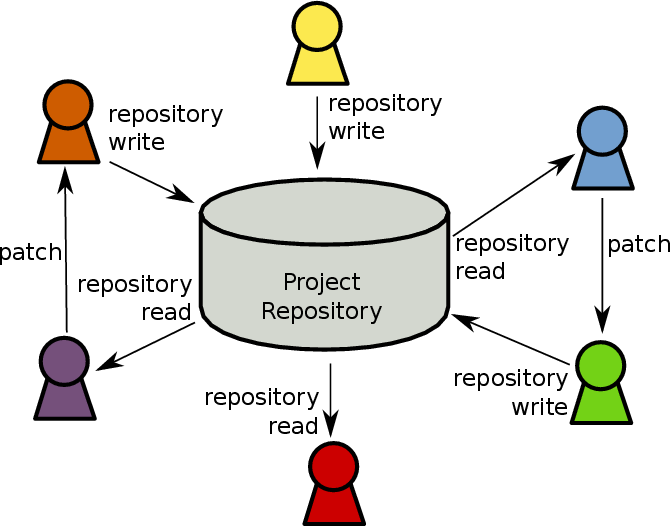
\includegraphics[scale=.95]{repository-interaction.png}
	    \caption{FLOSS development by means of a VCS repository}
	    \label{fig:background:free-software-repository}
	  \end{center}
	\end{figure}


        \begin{itemize}
		\item Source code availability: projects have a publicly-accessible version control repository
		\item User/developer symbiosis: the developers are also users of the software, and they
    also provide requirements
		\item Non-contractual work: there is no central management with control over all of the
    developers' activities
		\item Work is self-assigned: volunteer developers tend to work on the parts of
    the project that most appeal to them, and employed developers will
    work on the parts that are of most interest to their employers
		\item Geographical Distribution: in most FLOSS
    projects the developers are spread among several different locations
    in the world
	\end{itemize}
\end{block}


%-------------------------------------------------------------------------------
\vfill
\begin{block}{Opportunities}
	\begin{itemize}
		\item Using FLOSS for SE Education
		\begin{itemize}
			\item Involving students and faculty in large-scale FLOSS projects to provide them with real-world experience
			\item FLOSS promotes project- and problem-based learning, developers/students work on projects that interest them
			\item FLOSS is normally highly modular and APIs are well documented, for teaching principles and good practices
			\item Provides quantitative data from real and freely available source code on which to perform analysis and base decisions

		\end{itemize}
		\item Using data from FLOSS projects in SE Research
		\begin{itemize}
			\item The social structure of development communities
			\item Communication and workflow patterns in FLOSS projects
			\item Developer evolution and participation
			\item Attractiveness of FLOSS projects
			\item Attributes of the source code and their impact on project success
		\end{itemize}
		\item FLOSS software products in research activities
		\begin{itemize}
			\item Releasing the source of software produced in research activities meets the basic scientific principle of reproducibility
			\item Being open source allows research prototypes to be enhanced into production-class products without the researchers having to be involved forever
		\end{itemize}
	\end{itemize}
\end{block}

\vfill
        

}
\end{minipage}
\end{beamercolorbox}
\end{column}
% ---------------------------------------------------------%
% end the column

% ---------------------------------------------------------%
% Set up a column 
\begin{column}{.49\textwidth}
  \begin{beamercolorbox}[center,wd=\textwidth]{postercolumn}
    \begin{minipage}[T]{.95\textwidth} % tweaks the width, makes a new \textwidth
      \parbox[t][\columnheight]{\textwidth}{ % must be some better way to set the the height, width and textwidth simultaneously
        % Since all columns are the same length, it is all nice and tidy.  You have to get the height empirically
        % ---------------------------------------------------------%
        % fill each column with content

        \begin{block}{FLOSS in SBES (Brazil)}
          \begin{itemize}
          	\item 378 papers analyzed: 206 main track papers between 1999 and 2010, 142 tools session papers 
between 2001 and 2010, and 30 FEES papers from 2008 to 2010
          	\item Matchers: software(s) livre(s), ferramenta(s) livre(s), ferramenta(s) aberta(s), software(s) aberto(s), c�digo aberto, reposit�rio(s) de software, free software, open source, open software, libre software, software repository, OSS, FLOSS, FOSS, and OSSD
		\end{itemize}

	\begin{table}
		\begin{center}
		\caption{Main track papers analyzed, by year}
		\label{table:maintrack:papers-by-year}
		\begin{tabular}{rrrr}
		  \hline
		Year & Analyzed & Mention FLOSS & Relative frequency \\ 
		  \hline
		1999 &  26 &   0 & 0.00 \\ 
		  2001 &  20 &   0 & 0.00 \\ 
		  2002 &  18 &   2 & 0.11 \\ 
		  2004 &  17 &   1 & 0.06 \\ 
		  2005 &  21 &   2 & 0.10 \\ 
		  2006 &  19 &   0 & 0.00 \\ 
		  2007 &  23 &   2 & 0.09 \\ 
		  2008 &  19 &   1 & 0.05 \\ 
		  2009 &  24 &   6 & 0.25 \\ 
		  2010 &  19 &  11 & 0.58 \\ 
		   \hline
		\end{tabular}
		\end{center}
	\end{table}

	\begin{table}
	\begin{center}
	\caption{Analysis of research papers mentioning FLOSS}
	\label{table:maintrack-papers}
	\begin{tabular}{lrrrrrrr|r}
	  \hline
	    Category                & 2002 & 2004 & 2005 & 2007  & 2008  & 2009  & 2010  & Total \\
	  \hline
	    Reference               & 0    & 0    & 0    & 1     & 0     & 1     & 1     & 3 \\
	    Example or Comparison   & 1    & 0    & 0    & 0     & 0     & 1     & 1     & 3 \\
	    Running FLOSS tools     & 1    & 1    & 2    & 0     & 1     & 1     & 0     & 6 \\
	    FLOSS tool as target    & 0    & 0    & 0    & 1     & 0     & 0     & 3     & 4 \\
	    Data from FLOSS         & 0    & 0    & 0    & 0     & 0     & 2     & 3     & 5 \\
	    Research about FLOSS    & 0    & 0    & 0    & 0     & 0     & 1     & 3     & 4 \\
	  \hline
	    Total                   & 2    & 1    & 2    & 2     & 1     & 6     & 11    & 25 \\
	  \hline
	\end{tabular}
	\end{center}
	\end{table}

	\begin{table}[ht]
		\begin{center}
		\caption{Tool papers analyzed, by year}
		\label{table:tools:papers-by-year}
		\begin{tabular}{rrrr}
		  \hline
		Year & Analyzed & Mention FLOSS & Relative frequency \\ 
		  \hline
		2001 &  18 &   0 & 0.00 \\ 
		  2002 &  19 &   3 & 0.16 \\ 
		  2004 &  15 &   2 & 0.13 \\ 
		  2005 &  12 &   2 & 0.17 \\ 
		  2006 &  25 &   7 & 0.28 \\ 
		  2007 &  14 &   2 & 0.14 \\ 
		  2008 &  11 &   3 & 0.27 \\ 
		  2009 &  12 &   4 & 0.33 \\ 
		  2010 &  16 &   7 & 0.44 \\ 
		   \hline
		\end{tabular}
		\end{center}
	\end{table}

	\begin{table}
		\begin{center}
		\caption{Analysis of tools papers mentioning FLOSS}
		\label{table:tools-papers}
		\begin{tabular}{lrrrrrrrr|r}
		  \hline
		    Context                         & 2002 & 2004 & 2005  & 2006  & 2007  & 2008  & 2009  & 2010  & Total \\
		  \hline
		    Reference                       & 1    & 0    & 0     & 0     & 1     & 0     & 0     & 0     & 2 \\
		    Promise to be FLOSS             & 0    & 0    & 1     & 1     & 0     & 1     & 0     & 1     & 4 \\
		    use FLOSS                       & 1    & 1    & 0     & 0     & 0     & 0     & 1     & 1     & 4 \\
		    FLOSS (fake*)
						    & 0    & 1    & 0     & 5     & 1     & 2     & 2     & 3     & 14 \\
		    FLOSS                           & 1    & 0    & 1     & 1     & 0     & 0     & 1     & 2     & 6 \\
		  \hline
		    Total                           & 3    & 2    & 2     & 7     & 2     & 3     & 4     & 7     & 30 \\
		  \hline
		\end{tabular}
		\end{center}
	\end{table}

	 \begin{itemize}
          	\item The Brazilian Software Engineering community
could be taking more advantage of the FLOSS research opportunities
	 	\begin{itemize}
			\item We are late in comparison with the international scenario 
		\end{itemize}
	\end{itemize}

        \end{block}
             
	\vfill
\begin{block}{Agenda}
          \begin{itemize}

			\item Public Data: Encouraging that software research uses public data and FLOSS tools
    to process and analyze data

			\item Venues: Increase the number of venues welcoming results from FLOSS research

			\item Tools: Creating a repository for publishing the FLOSS tools presented in the tools
    sessions of Brazilian software engineering conferences and workshops

			\item Educational Material: creating a repository of educational material and a forum where SE educators can discuss and share
    experiences in the use of FLOSS (see: \textbf{softwarelivre.org/sbc})

			\item FLOSSCC: Fostering the creation of FLOSS Competence Centers throughout the
    country

          \end{itemize}
        \end{block}
\vfill
      }
      % ---------------------------------------------------------%
      % end the column
        \end{minipage}
      \end{beamercolorbox}
    \end{column}
    % ---------------------------------------------------------%
    % end the column
  \end{columns}
  %\vskip1ex
  % \tiny\hfill\textcolor{ta2gray}{Created with \LaTeX \texttt{beamerposter}  \url{http://www-i6.informatik.rwth-aachen.de/~dreuw/latexbeamerposter.php}}
  
\end{frame}
\end{document}


%%%%%%%%%%%%%%%%%%%%%%%%%%%%%%%%%%%%%%%%%%%%%%%%%%%%%%%%%%%%%%%%%%%%%%%%%%%%%%%%%%%%%%%%%%%%%%%%%%%%
%%% Local Variables: 
%%% mode: latex
%%% TeX-PDF-mode: t
%%% End:

% LocalWords:  ABox ABoxes PSAT
